% -*-coding: utf-8 -*-
\defaultfont
\BiChapter{水下绳驱机械臂结构研制}{Structural Development of Underwater Cable-Driven Robotic Arm}
\label{Tricks}

\BiSection{引言}{Introduction}
\label{tricks:abouttemplates}
本章面向水下抓取作业需求，研制了一款水下绳驱机械臂。该机械臂采用绳驱动结构，将质量较大的驱动电机后置于基座，从而有效减小运动过程中对运载器的扰动。为此，本章围绕绳驱机械臂的结构设计展开研究，具体内容包括：总体方案设计、本体结构设计、驱动绳走线分析及驱动密封舱设计。

\BiSection{水下绳驱机械臂设计要求}{Design Requirements}
针对搭载于微小型运载器的对海底作业机械臂，设计时需满足以下要求：
(1) 机械臂安装于运载器正下方，能够实现完全折叠收拢；
(2) 机械臂完全伸展下探深度需大于 500mm；
(3) 机械臂运动部分总重量不大于 3kg；
(4) 机械臂需具备 1kg 的有效负载能力。

\BiSection{机械臂总体结构设计}{Overall Structural Design}
\BiSubsection{机械臂总体方案设计}{General Scheme Design}
\label{tricks:necessaryornot}
为兼顾小型化与低扰动设计需求，本文设计的绳驱方案采用驱动集成化策略，将动力源安置于单一密封舱内。针对多自由度带来的精度衰减问题，本文采用 3 自由度（肩部水平转动、肘部俯仰、腕部俯仰）构型，其基本机构简图如图 \ref{pic12} 所示。

\begin{figure}[H]
    \centering
    
\includegraphics[width = 0.7\textwidth]{机构简图1}
    \caption{绳驱机械臂机构简图}
    \label{pic12}
\end{figure}

为实现完全折叠归位，本文设计了一种关联双铰链滚动机构以改进肘部关节。该结构扩展了关节的可折叠空间，使大臂在非工作状态下能完全嵌套于载体下方，有效降低了巡航阻力。改进后的结构如图 \ref{pic13} 所示。

\begin{figure}[H]
    \centering
    
\includegraphics[width = 0.8\textwidth]{机构简图2}
    \caption{可折叠绳驱机械臂机构简图}
    \label{pic13}
\end{figure}

\BiSubsection{机械臂本体结构设计}{Mechanical Body Design}
(1) 关节 1 水平旋转关节设计

水平旋转关节采用基于欧拉绞盘原理的单绳循环驱动方案，其原理如图 \ref{pic14} 所示。
\begin{itemize}
    \item \textbf{驱动原理与缠绕逻辑}：如图 \ref{pic14} 所示，驱动绳在驱动轴上采取“一端正绕、一端反绕”配置，通过电机的旋转实现绳索的等量收放，从而驱动关节绞盘同步转动。
    \begin{figure}[H]
        \centering
        
\includegraphics[width = 0.6\textwidth]{f1}
        \caption{水平旋转关节原理图}
        \label{pic14}
    \end{figure}
    \item \textbf{防滑设计}：利用绞盘方程 $T_{load} = T_{hold} \cdot e^{\mu\phi}$，通过增加驱动绳在绞盘上的缠绕圈数（增大包角 $\phi$），可以在低初始张力下获得较大摩擦力，避免打滑。
\end{itemize}

(2) 关节 2 肘部双铰链滚动关节

肘部关节集成了滑轮组倍率放大机构，其具体结构分布如图 \ref{fig:total_figure2} 所示。

\begin{figure}[H]
  \centering
  \begin{minipage}{\textwidth}
      \centering
      \subfigure[肘部关节外侧结构]{\label{fig:sub1}
      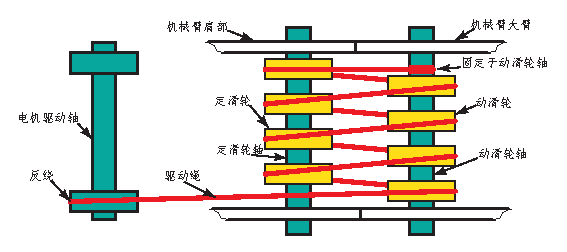
\includegraphics[width = 0.8\textwidth]{figures/动滑轮.eps}}
  \end{minipage}
  \begin{minipage}{\textwidth}
      \centering
      \subfigure[肘部关节内侧结构]{\label{fig:sub2}
      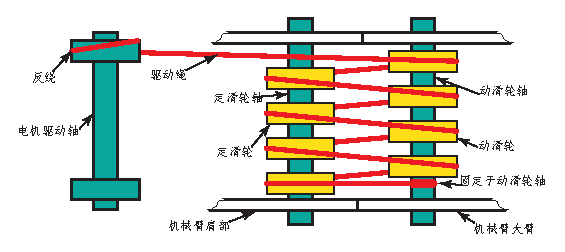
\includegraphics[width = 0.8\textwidth]{figures/动滑轮2.eps}}
  \end{minipage}
  \caption{肘部关节增力传动机构详图}
  \label{fig:total_figure2}
\end{figure}

该关节采用纯滚动接触面设计。图 \ref{fig:total_figure3} 展示了该关节在运动过程中的两种状态：完全伸展态与极限位置态。

\begin{figure}[H]
  \centering
  \begin{minipage}{0.48\textwidth}
      \centering
      \subfigure[完全伸展状态]{\label{fig:3sub1}
      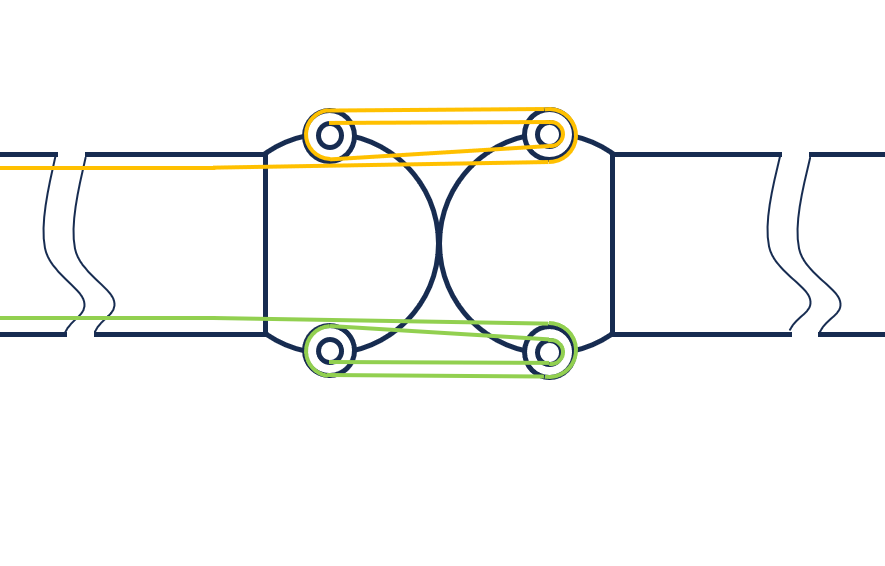
\includegraphics[width=\textwidth]{figures/伸展.png}}
  \end{minipage}
  \hfill
  \begin{minipage}{0.48\textwidth}
      \centering
      \subfigure[极端位置状态]{\label{fig:3sub2}
      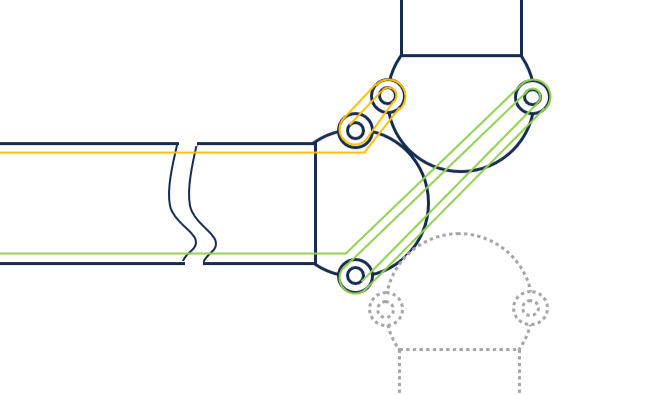
\includegraphics[width=\textwidth]{figures/极端.png}}
  \end{minipage}
  \caption{关节 2 肘部运动状态示意图}
  \label{fig:total_figure3}
\end{figure}

为满足收纳要求，滑轮组采用斜向布局，消除了结构干涉。其收拢与折叠效果如图 \ref{fig:total_figure4} 所示。

\begin{figure}[H]
    \centering
    \begin{minipage}{0.48\textwidth}
        \centering
        \subfigure[收拢位置姿态]{\label{fig:4sub1}
        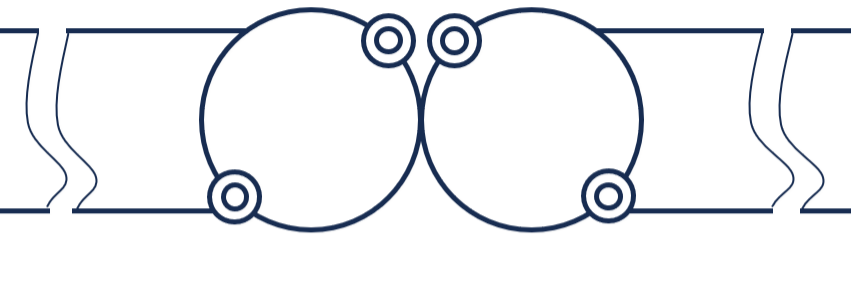
\includegraphics[width=\textwidth]{figures/收拢位置.png}}
    \end{minipage}
    \hfill
    \begin{minipage}{0.48\textwidth}
        \centering
        \subfigure[完全折叠状态]{\label{fig:4sub2}
        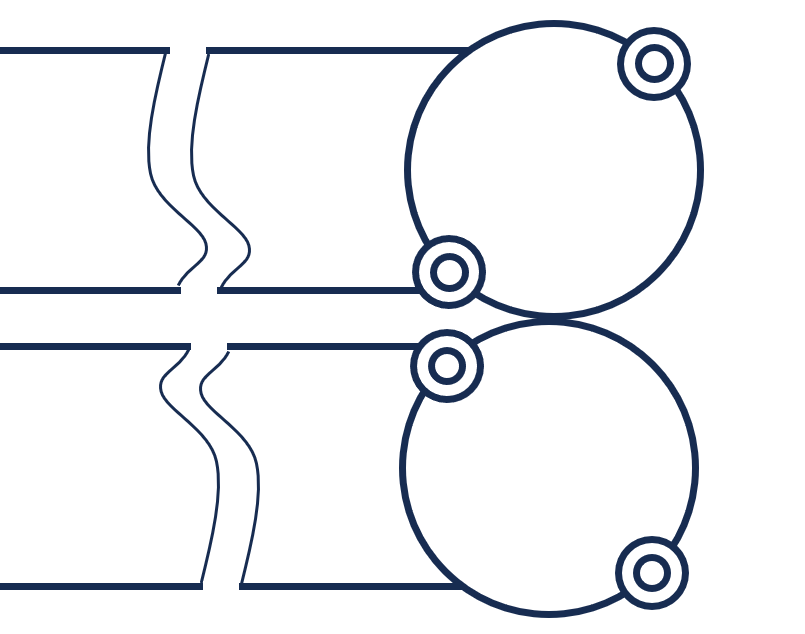
\includegraphics[width=\textwidth]{figures/折叠位置.png}}
    \end{minipage}
    \caption{关节 2 可折叠方案展示}
    \label{fig:total_figure4}
\end{figure}

此外，设计了如图 \ref{fig:total_figure5} 所示的机械硬限位结构，将肘部旋转角度限制在 $0^\circ \sim 180^\circ$。

\begin{figure}[H]
    \centering
    \begin{minipage}{0.48\textwidth}
        \centering
        \subfigure[伸展限位]{\label{fig:5sub1}
        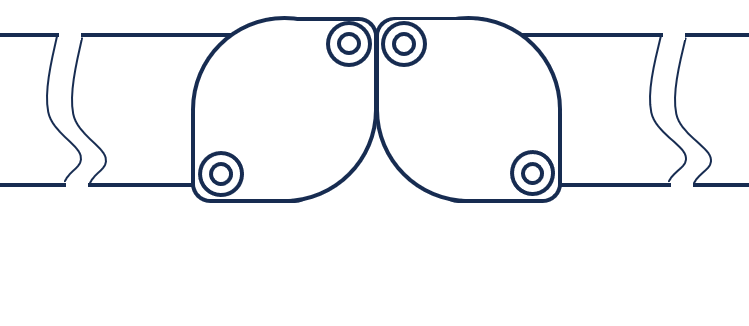
\includegraphics[width=\textwidth]{figures/最大工作.png}}
    \end{minipage}
    \hfill
    \begin{minipage}{0.48\textwidth}
        \centering
        \subfigure[折叠限位]{\label{fig:5sub2}
        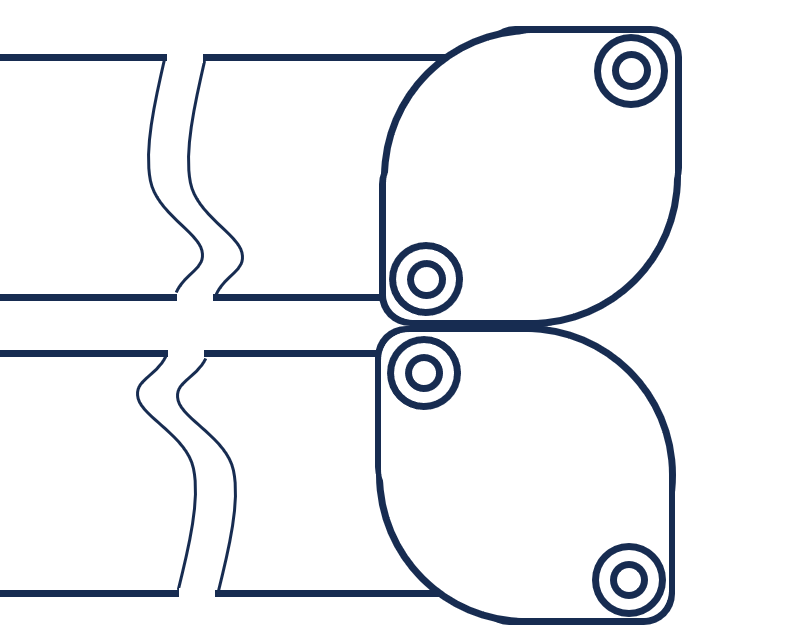
\includegraphics[width=\textwidth]{figures/最小工作.png}}
    \end{minipage}
    \caption{肘部机械限位结构图}
    \label{fig:total_figure5}
\end{figure}

(3) 总体装配效果

基于上述设计，绳驱机械臂的三维结构及不同作业姿态如图 \ref{fig:total_figure6} 所示。其中，图 \ref{fig6:sub2} 展示了最大下探深度可达 730mm。

\begin{figure}[H]
    \centering
    \begin{minipage}{\textwidth}
        \centering
        \subfigure[完全折叠状态]{\label{fig6:sub1}
        \includegraphics[width = 0.6\textwidth]{figures/完全收拢.jpg}}
    \end{minipage}
    \begin{minipage}{\textwidth}
        \centering
        \subfigure[完全下探状态]{\label{fig6:sub2}
        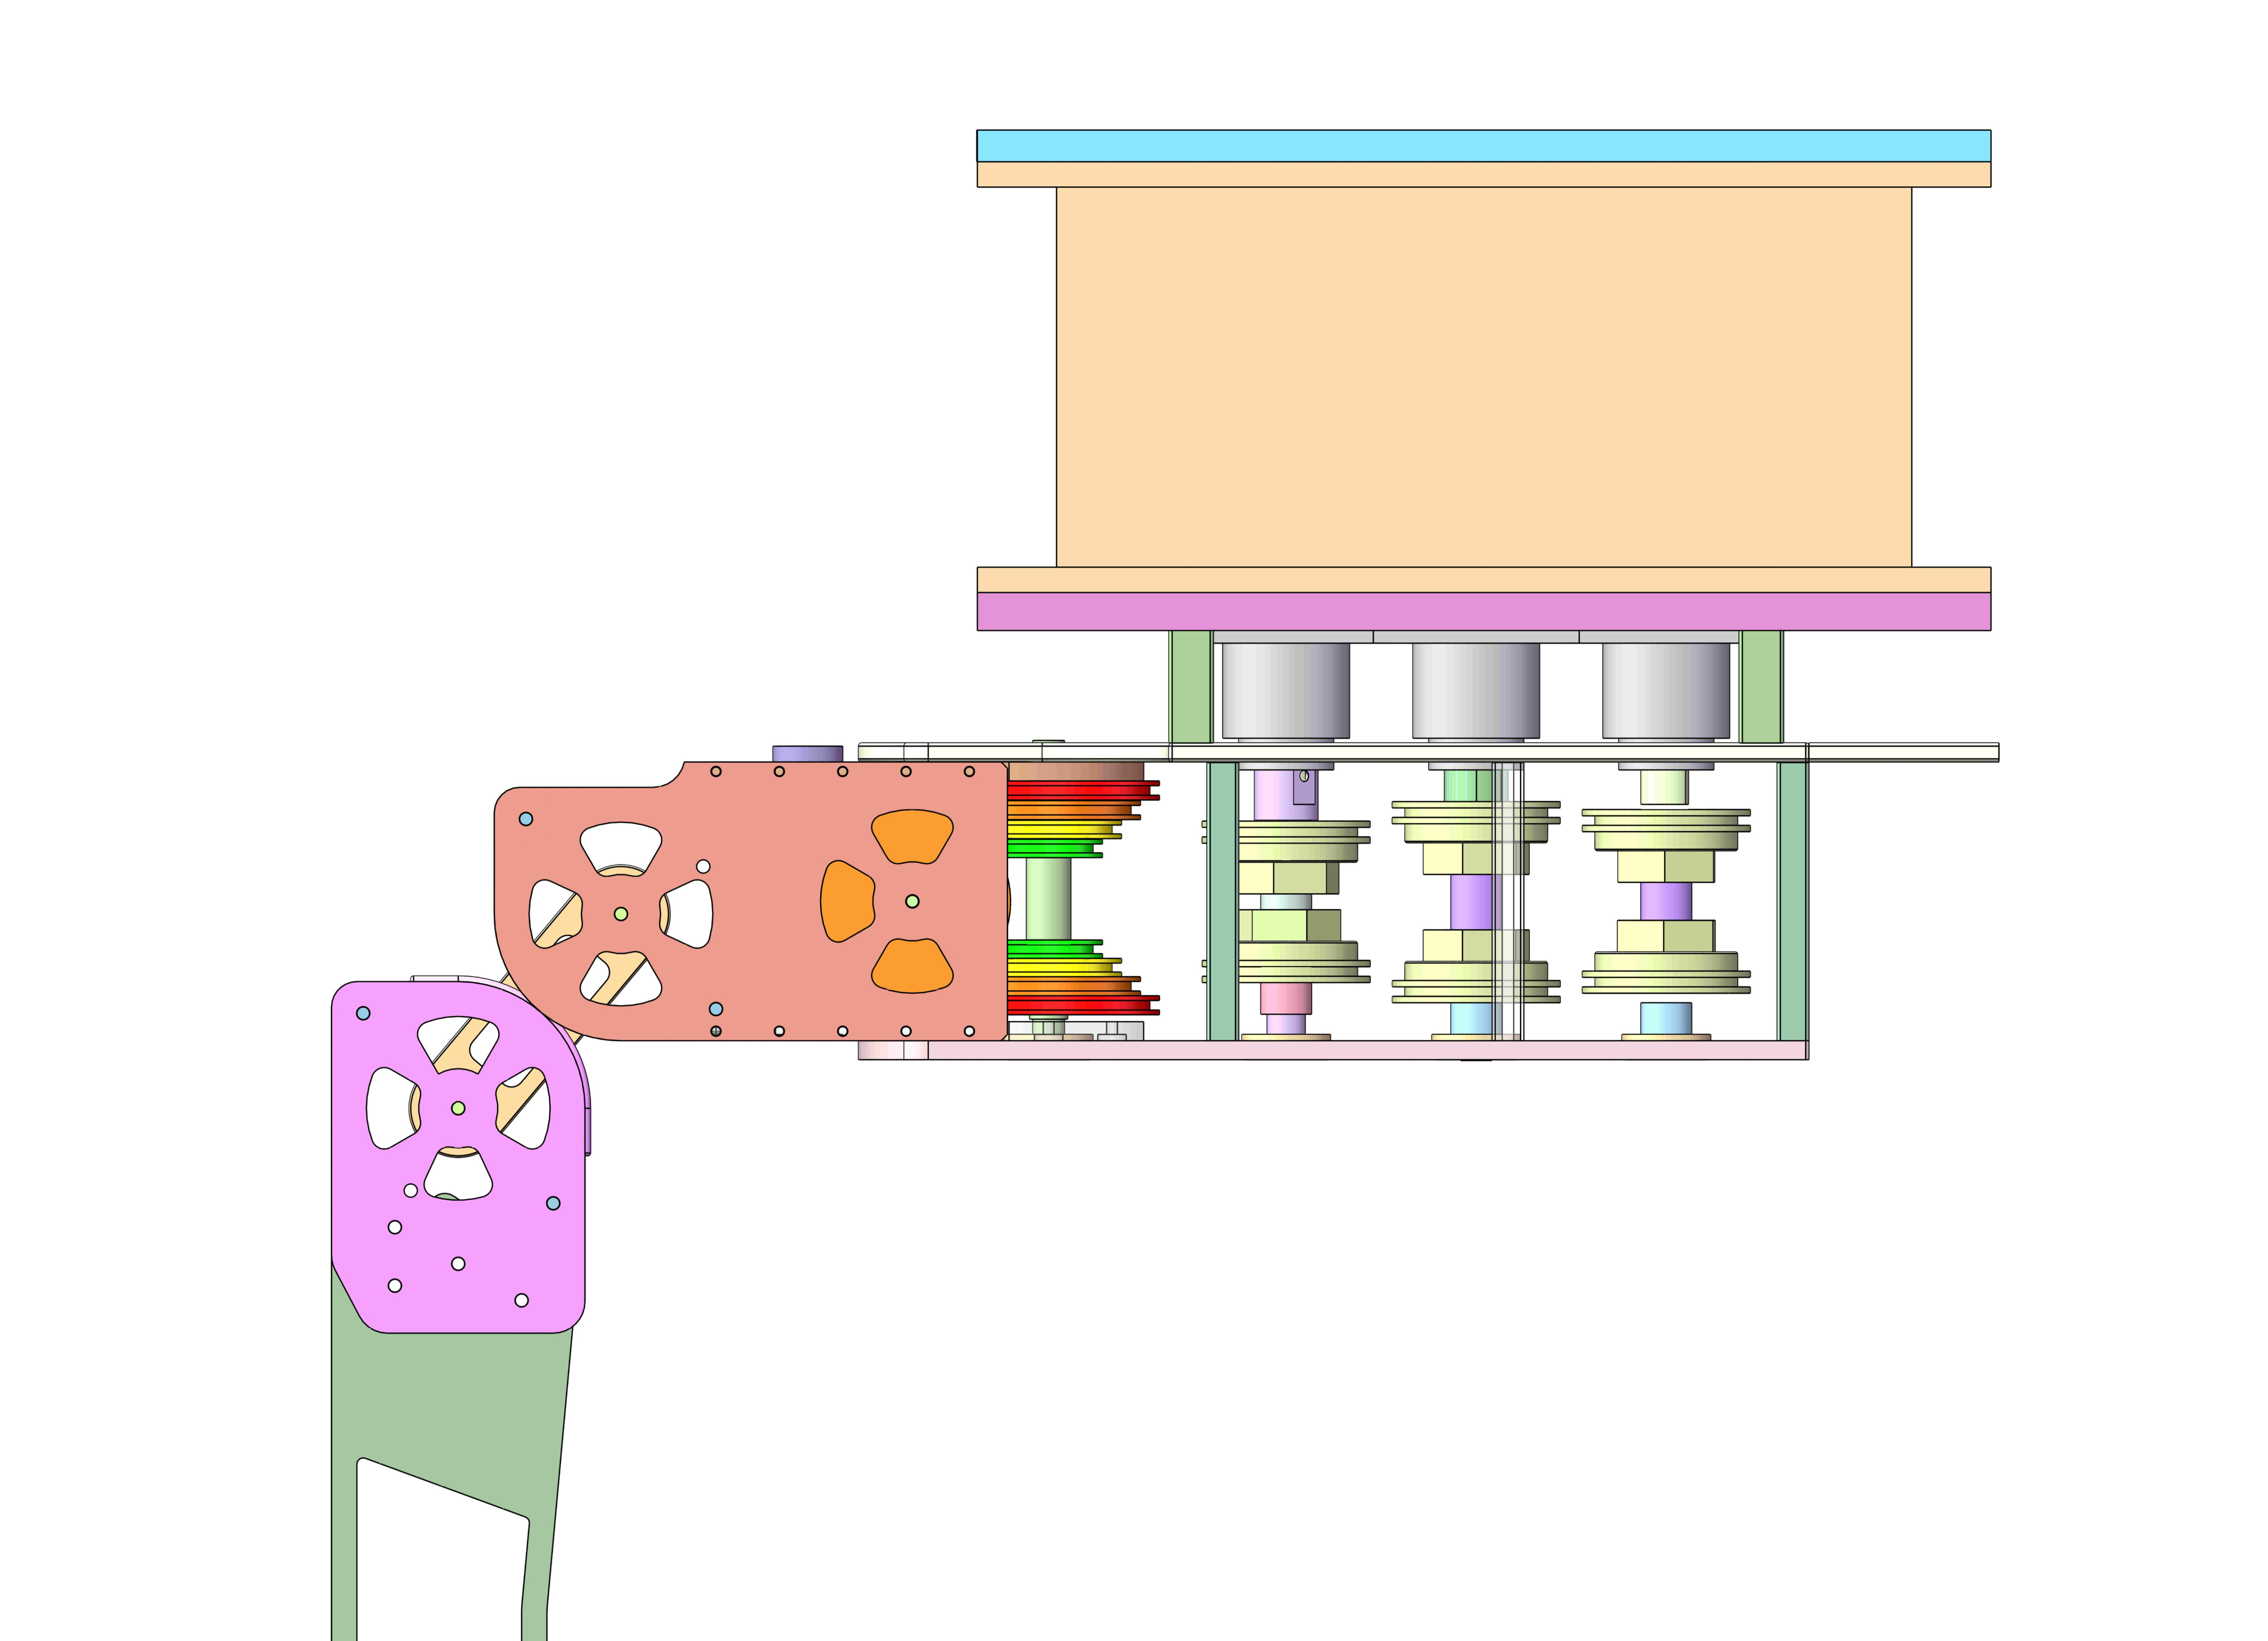
\includegraphics[width = 0.6\textwidth]{figures/下探姿态.jpg}}
    \end{minipage}
    \caption{机械臂多姿态装配示意图}
    \label{fig:total_figure6}
\end{figure}

\BiSubsection{驱动绳走线及导向设计}{Cable Routing and Guiding Design}
本节选用滑轮导向方案，滑轮的基本力学与运动特性参考图 \ref{pic23}。

\begin{figure}[H]
    \centering
    
\includegraphics[width = 0.25\textwidth]{滑轮原理}
    \caption{滑轮导向特性示意图}
    \label{pic23}
\end{figure}

肩关节及肘关节的具体走线布局分别如图 \ref{pic24} 及图 \ref{fig:total_figure8} 所示。
\begin{figure}[H]
    \centering
    \includegraphics[width = 0.7\textwidth]{肩关节导}
    \caption{肩关节导向结构走线图}
    \label{pic24}
\end{figure}

\begin{figure}[H]
    \centering
    \subfigure[肘部外侧走线]{\label{fig8:sub1}
    \includegraphics[width = 0.45\textwidth]{figures/肘部外侧走线.eps}}
    \hfill
    \subfigure[肘部内侧走线]{\label{fig8:sub2}
    \includegraphics[width = 0.45\textwidth]{figures/肘关节内侧走线(1).eps}}
    \caption{肘部关节复杂走线导向图}
    \label{fig:total_figure8}
\end{figure}

针对绳索松弛问题，设计了基于双向自锁原理的张紧机构，结构详见图 \ref{fig:total_figure9}。
\begin{figure}[H]
    \centering
    \subfigure[张紧机构实物]{\label{fig9:sub1}
    \includegraphics[width = 0.45\textwidth]{figures/装配体3轴(1).eps}}
    \hfill
    \subfigure[张紧机构剖视]{\label{fig9:sub2}
    \includegraphics[width = 0.45\textwidth]{figures/装配体3轴1(1).eps}}
    \caption{绳索张紧机构设计}
    \label{fig:total_figure9}
\end{figure}

\BiSubsection{驱动系统密封舱设计}{Drive System Pressure Housing Design}
驱动密封舱内部集成了控制单元与电机，具体组件参数详见表 \ref{tab:cabin_components}。核心动力与控制硬件如图 \ref{fig:total_figure11} 及图 \ref{fig:total_figure13} 所示。

% ... 表格保持不变 ...

\begin{figure}[H]
    \centering
    \subfigure[Faulhaber 电机]{\label{fig11:sub1}
    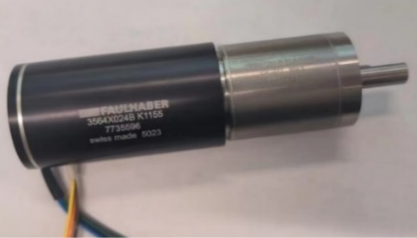
\includegraphics[width = 0.45\textwidth]{figures/电机.png}}
    \hfill
    \subfigure[配套驱动器]{\label{fig11:sub2}
    
\includegraphics[width = 0.4\textwidth]{figures/驱动.png}}
    \caption{动力驱动单元}
    \label{fig:total_figure11}
\end{figure}

在密封设计方面，静密封（O型圈、水密插件）与动密封（格莱圈、分体式组件）的结构设计分别如图 \ref{fig:total_figure16} 与 \ref{fig:total_figure15} 所示。

\begin{figure}[H]
    \centering
    \subfigure[O型密封圈]{\label{fig16:sub1}
    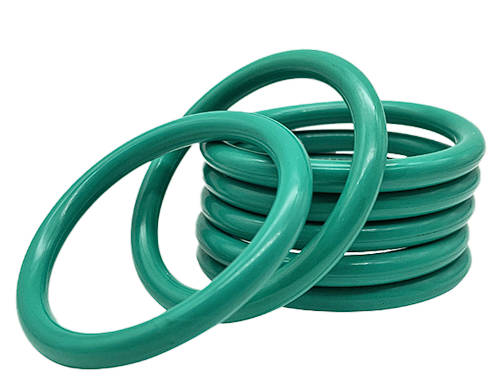
\includegraphics[width = 0.4\textwidth]{figures/oring.jpg}}
    \hfill
    \subfigure[水密接插件布局]{\label{fig16:sub2}
    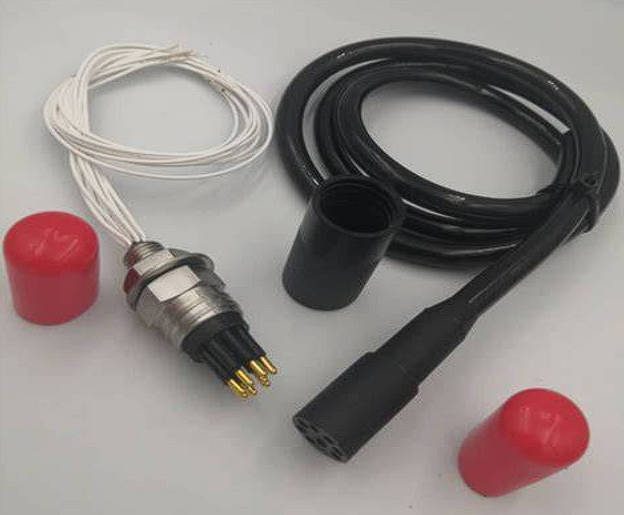
\includegraphics[width = 0.4\textwidth]{figures/接插件.jpg}}
    \caption{密封舱静密封组件}
    \label{fig:total_figure16}
\end{figure}

\begin{figure}[H]
    \centering
    \subfigure[旋转轴用格莱圈]{\label{fig15:sub1}
    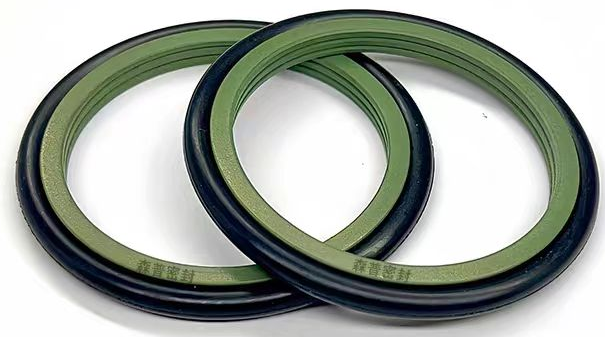
\includegraphics[width = 0.4\textwidth]{figures/格莱圈.png}}
    \hfill
    \subfigure[分体式动密封组件]{\label{fig15:sub2}
    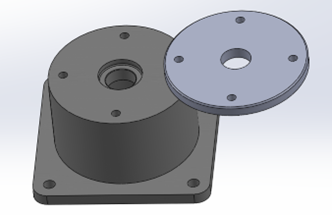
\includegraphics[width = 0.4\textwidth]{figures/组件.png}}
    \caption{电机输出轴动密封方案}
    \label{fig:total_figure15}
\end{figure}

密封舱的整机装配与内部布局最终如图 \ref{pic26} 所示。
\begin{figure}[H]
    \centering
    
\includegraphics[width = 0.8\textwidth]{内部布局}
    \caption{机械臂密封舱内部结构布局图}
    \label{pic26}
\end{figure}

\BiSection{水下绳驱机械臂样机集成}{Prototype Integration}
集成完成后的水下绳驱机械臂样机实物如图 \ref{fig:total_figure18} 所示。样机总质量为 1.8kg，实现了从完全折叠到最大下探姿态的平稳切换。

\begin{figure}[H]
    \centering
    \subfigure[样机轴测图]{\label{fig18:sub1}
    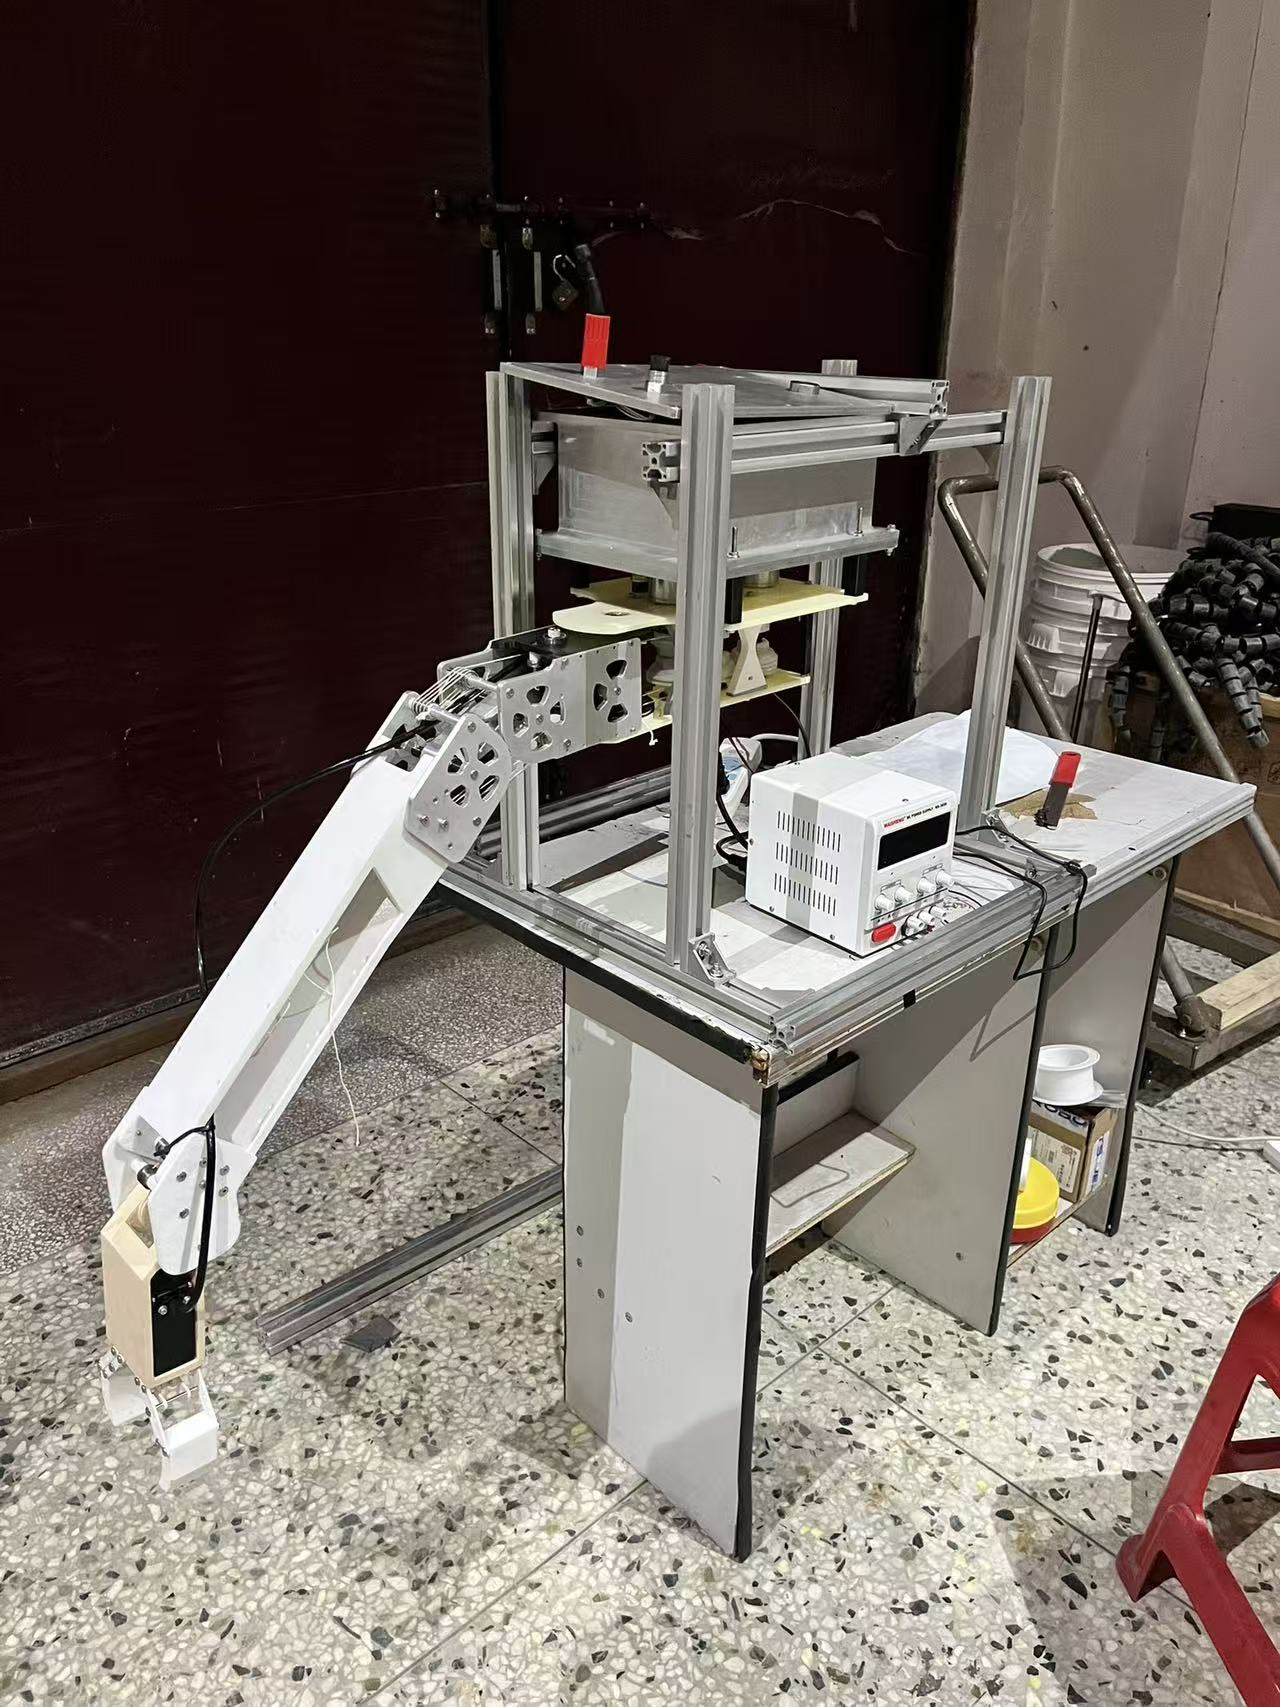
\includegraphics[width = 0.45\textwidth]{figures/轴测图.jpg}}
    \hfill
    \subfigure[样机侧视图]{\label{fig18:sub2}
    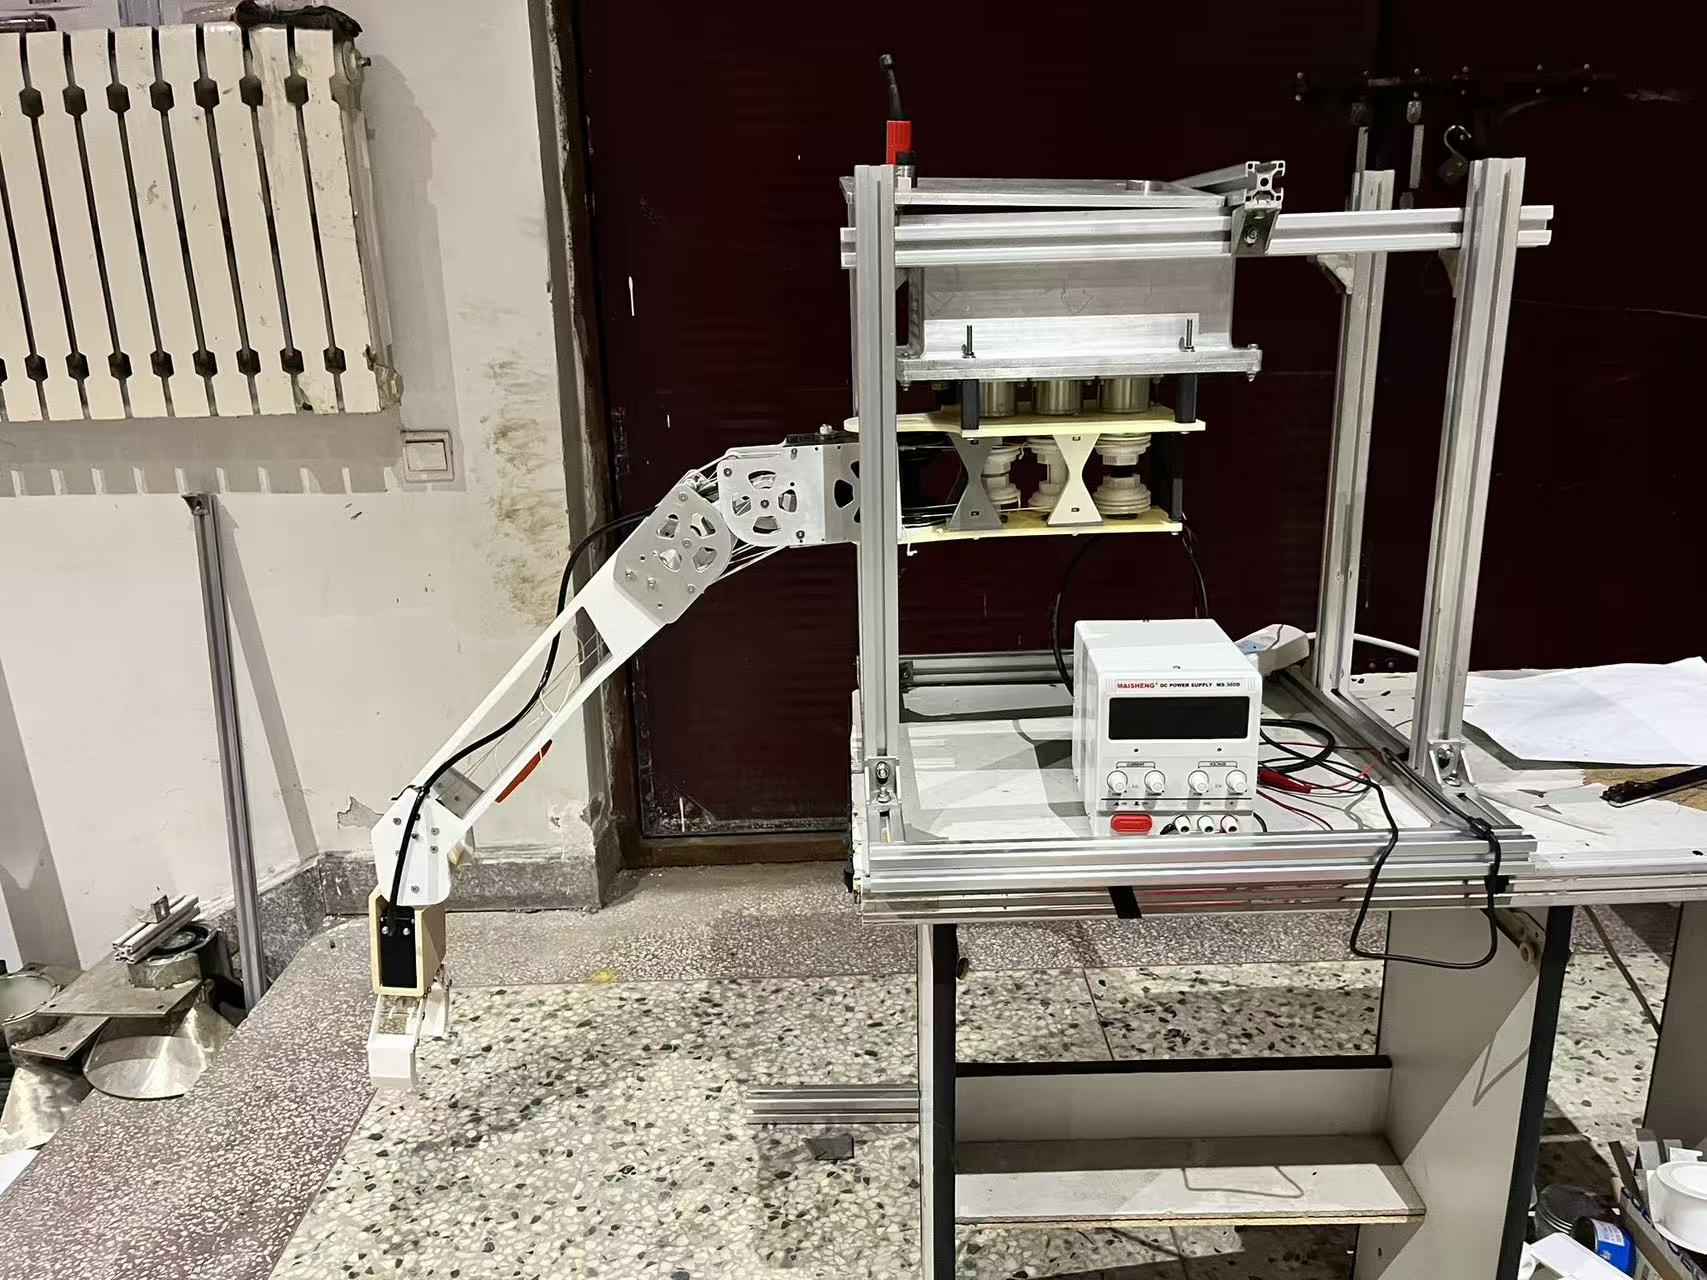
\includegraphics[width = 0.48\textwidth]{figures/侧视图.jpg}}
    \caption{水下绳驱机械臂样机实物}
    \label{fig:total_figure18}
\end{figure}

\BiSection{本章小结}{Summary}
本章完成了一款三自由度水下绳驱机械臂的研制，实现了完全折叠构型、滑轮组增力传动及可靠的高压密封设计，为后续运动学建模与控制研究奠定了硬件基础。